\begin{figure}[H]
    \centering
    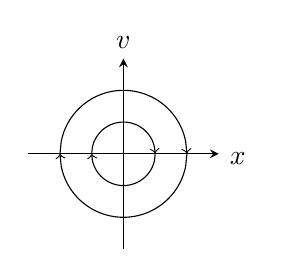
\begin{tikzpicture}
	\begin{axis}[
	    width=4cm,
	    height=4cm,
	    xmin= -3, xmax= 3,
	    ymin= -3, ymax = 3,
	    axis lines = middle,
	    x label style={at={(axis description cs:1.1,0.56)},anchor=north},
	    y label style={at={(axis description cs:0.5,1)},anchor=south},
	    xlabel={$x$},
	    ylabel={$v$},
	    xtick={0},
	    ytick={0},
	    xticklabel={},
	    yticklabel={},
	    ]

	    \addplot [domain=-2:2, samples=100, ->] {sqrt(4-x^2)};
	    \addplot [domain=-2:2, samples=100, <-] {-sqrt(4-x^2)};

	    \addplot [domain=-1:1, samples=100, ->] {sqrt(1-x^2)};
	    \addplot [domain=-1:1, samples=100, <-] {-sqrt(1-x^2)};

	\end{axis}
    \end{tikzpicture}
    \caption{\scriptsize Moto nello spazio delle fasi per un oscillatore armonico.}
    \label{fig:osc_armonico}
\end{figure}
